%versi 2 (8-10-2016)
\chapter{Landasan Teori}
\label{chap:teori}


 
Pada bab ini akan dibahas mengenai landasan teori yang digunakan pada penyusunan tugas akhir. Pembahasan pertama mencakup hal-hal yang berkaitan dengan pengertian kewirausahaan dari umum sampai khusus yaitu kewirausahaan menurut GEM. Pembahasan kedua yaitu tentang teori dan aplikasi dari CA (Cellular Automata) khususnya tentang ECA (Entrepreneurial Cellular Automata). Pembahasan terakhir tentang graf.


\section{Arti Kewirausahaan}
\label{sec:artiwirausaha}

\graphicspath{{images/}}

Wirausaha berasal dari kata wira dan usaha. Wira artinya unggul, mulia, luhur sedangkan usaha berarti kemampuan melakukan usaha atas kekuatan diri sendiri. Jadi wirausaha adalah manusia yang unggul yang memiliki kemampuan membangun usaha sendiri. Kewirausahaan sendiri merupakan kepribadian wirausaha. Wirausaha merupakan orang atau manusia yang memperjuangkan kemajuan terutama pada bidang ekonomi demi masyarakat seperti menciptakan lapangan pekerjaan, membantu memenuhi kebutuhan masyarakat yang semakin meningkat dan berusaha mengurangi ketergantungan dari luar negeri. Istilah kewirausahaan pada umumnya merupakan suatu ilmu yang mempelajari tentang kemampuan seseorang dalam menghadapi tantangan hidup untuk memperoleh peluang dan menghadapi segala risiko yang ada dengan mengandalkan kekuatan diri sendiri tanpa bergantung pada orang lain. \cite{artiwirausaha} 


%Kewirausahaan menurut GEM merupakan proses yang terdiri dari fase-fase berbeda mulai dari niat mendirikan suatu usaha, menjalankan suatu usaha baru atau sudah berdiri dan sampai usaha tersebut berhenti. Proses ini dimulai dengan keterlibatan individu yang berpotensi untuk menjadi wirausaha, yaitu mereka yang percaya bahwa mereka mempunyai kemampuan untuk memulai suatu usaha, individu yang melihat kesempatan untuk berwirausaha dan individu yang tidak takut gagal dalam memulai suatu usaha. \cite{wirausahaGEM}
GEM (Global Entrepreneurship Monitor) merupakan lembaga yang memantau dan mengukur pertumbuhan wirausaha di berbagai negara yang didirikan pada tahun 1997 oleh Michael Hay dan Bill Bygrave. GEM telah memantau kewirausahaan di 104 ekonomi negara dan telah mendapat pengakuan luas sebagai penelitian kewirausahaan secara longitudinal yang memiliki kewenangan kuat di dunia . Pada tahun 2006, Indonesia sempat bergabung dengan GEM untuk mempelajari kewirausahaan. Setelah absen selama 6 tahun, Indonesia kembali bergabung dengan GEM pada tahun 2013.\cite{ECA}


GEM melakukan penelitiannya berdasarkan pada beberapa premis. Pertama, keadaan ekonomi suatu negara. Jika keadaan ekonomi suatu negara sedang sulit itu artinya dengan adanya wirausaha dapat membantu memperluas lapangan pekerjaan (memotivasi orang untuk menjadi seorang wirausaha juga lebih meningkat), sedangkan jika keadaan ekonomi suatu negara sudah baik keberadaan wirausaha tidak terlalu dibutuhkan (memotivasi orang untuk menjadi seorang wirausaha sudah kurang menarik). Kedua, kemampuan dan motivasi individu untuk memulai sebuah usaha dan pandangan masyarakat tentang wirausaha. Ketiga, pertumbuhan tinggi kewirausahaan dan persaingan antar negara tentang seberapa inovatif usaha tersebut. \cite{GEM2013}

Kewirausahaan menurut GEM merupakan sebuah proses yang memiliki tahapan-tahapan yang berbeda (Gambar \ref{fig:fasewirausaha}). Tahapan-tahapannya antara lain adalah dimulai dari niat mendirikan usaha, menjalankan usaha dan yang terakhir adalah berhentinya usaha yang dibuat. Tahapan pertama yaitu wirausaha \textit{potential}. Wirausaha \textit{potential} merupakan individu yang berpotensi untuk menjadi wirausaha, mereka percaya bahwa mereka memiliki kemampuan untuk memulai usaha, individu yang melihat kesempatan untuk berwirausaha, dan individu yang tidak takut gagal dalam memulai suatu usaha. Tahapan kedua yaitu wirausaha \textit{nascent}. Wirausaha \textit{nascent} ini merupakan tahapan dimana seseorang memulai usahanya dalam waktu kurang dari tiga bulan. Tahapan ketiga yaitu wirausaha \textit{new business owner}. Wirausaha \textit{new business owner} merupakan wirausaha \textit{nascent} yang usia bisnisnya sudah lebih dari 3 bulan tetapi kurang dari tiga tahun.

\begin{figure} [H]
	\centering  
	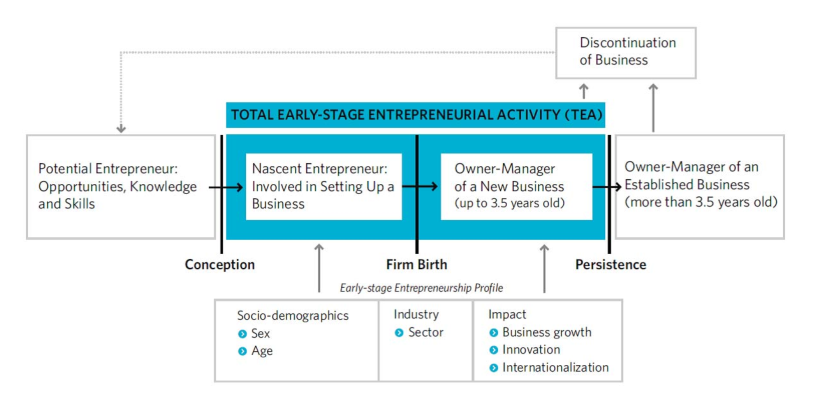
\includegraphics[width=16cm, height=10cm]{faseWirausaha}  
	\caption[Fase Wirausaha]{Fase Wirausaha} 
	\label{fig:fasewirausaha} 
\end{figure}

Wirausaha \textit{nascent} dan wirausaha \textit{new business owner} masuk ke dalam TEA (Total Early-Stage Entrepreneurial Activity). TEA merupakan persentase populasi antara usia 18 sampai 64 tahun yang berada pada tahap memulai usaha maupun pemilik bisnis yang waktunya kurang dari 42 bulan \cite{GEM2017}. Tahapan terakhir adalah wirausaha \textit{established} yaitu seseorang yang sudah menjalankan usahanya lebih dari tiga tahun dan tentunya sudah bisa menggaji orang.\cite{GEM2013}

Di setiap fase terdapat kemungkinan seorang wirausaha berhenti menjalankan usahanya. Berbagai faktor dapat mempengaruhi keberlangsungan wirausaha ini, diantaranya yaitu kondisi sosio-demografi, sektor industri, pertumbuhan wirausaha, inovasi,dll. Terdapat dua tipe atribut internal yang dimiliki setiap wirausahawan. Tipe pertama yaitu atribut umum seperti umur, pendapatan, pendidikan, bidang usaha, dll. Tipe kedua yaitu atribut individual dari GEM yang digunakan sebagai indikator kewirausahaan \cite{ECA}. Penjelasan beberapa indikator akan dijelaskan pada tabel \ref{tabelindikator2} dan tabel \ref{tabelindikator3}


\begin{table}[H]
\centering
\caption{Indikator Kewirausahaan}
\begin{tabular}{|p{4cm}|p{10cm}|}
\hline
Indikator & Deskripsi\\
\hline
New Product Early-stage Entrepreneurial (TEA) Activity & persentase dari TEA yang mengindikasikan bahwa produk atau jasa mereka masih baru\\
\hline
Growth Expectation Early-stage Entrepreneurial Activity : Relative Prevalence & persentase dari TEA yang berharap untuk meperkerjakan paling sedikit lima karyawan dalam waktu lima tahun kedepan\\
\hline
Informal Investors Rate & persentase dari populasi berusia 18-64 yang telah menyediakan dana untuk sebuah usaha baru, didirikan oleh orang lain, dalam waktu 3 tahun terakhir.\\
\hline
Total Early-stage Entrepreneurial Activity for Female Working Age Population & persentase dari populasi wanita berusia 18-64 yang antara lain merupakan seorang wirausaha \textit{nascent} atau pemilik manager dari sebuah usaha baru.\\
\hline
Total Early-stage Entrepreneurial Activity for Male Working Age Population & persentase dari populasi pria berusia 18-64 yang antara lain merupakan seorang wirausaha \textit{nascent} atau pemilik manager dari sebuah usaha baru.\\
\hline
Improvement-Driven Opportunity Entrepreneurial Activity : Relative Prevalence & persentase orang yang terlibat dalam TEA yang mengklaim bahwa mereka didorong oleh kesempatan, bukan karena kurangnya pilihan pekerjaan.\\
\hline
Necessity-Driven Entrepreneurial Activity : Relative Prevalence & persentase orang yang terlibat dalam TEA yang berwirausaha karena mereka tak punya pilihan pekerjaan lain\\
\hline
Established Business Ownership Rate & Persentase dari populasi berusia 18-64 yang merupakan pemilik manager dari sebuah usaha mapan dan sudah menghasilkan gaji atau untung apapun ke pemiliknya selama lebih dari 42 bulan.\\
\hline
Total Early-stage Entrepreneurial Activity & persentase dari populasi berusia 18-64 yang merupakan wirausaha nascent.\\
\hline
New Business Ownership Rate & Persentase dari populasi 18-64 yang merupakan pemilik manager dari sebuah usaha mapan yang sudah menghasilkan gaji atau untung selama lebih dari 3 bulan tetapi tidak lebih dari 42 bulan.\\
\hline
Nascent Entrepreneurship Rate & Persentase dari populasi 18-64 yang merupakan wirausaha nascent terlibat secara aktif memulai suatu usaha yang mereka miliki sendiri/bersama.\\
\hline
Media Attention for Entrepreneurship & persentase dari populasi berusia 18-64 yang setuju dengan pernyataan bahwa di negara mereka, mereka sering melihat atau mendengar di media tentang usaha baru yang sukses.\\
\hline
High status successful Entrepreneur & persentase dari populasi berusia 18-64 yang setuju dengan pernyataan bahwa di negara mereka, wirausaha yang sukses dihormati dan bercitra tinggi.\\
\hline
Entrepreneurship as Desirable Care & persentase dari populasi berusia 18-64 yang setuju dengan pernyataan bahwa di negara mereka, kebanyakan orang mempertimbangkan untuk memulai usaha baru sebagai karir yang diinginkan.\\
\hline
Know Startup Entrepreneur Rate (Role Model)& persentase dari populasi berusia 18-64 yang kenal seseorang yang mendirikan suatu usaha dalam waktu 2 tahun terakhir secara pribadi.\\
\hline
\end{tabular}
\label{tabelindikator2}
\end{table}

\begin{table} [H]
\centering
\caption{Lanjutan Indikator Kewirausahaan}
\begin{tabular}{|p{4cm}|p{10cm}|}
\hline
Entrepreneurial Intention & persentase dari populasi berusia 18-64 (individu yang terlibat dalam kegiatan wirausaha tidak termasuk) yang bertekad untuk mendirikan suatu usaha dalam waktu tiga tahun kedepan\\
\hline
Fear of Failure Rate & persentase dari populasi berusia 18-64 dengan perceived opportunities yang positif mengindikasikan bahwa takut pada kegagalan dapat menghambat mereka dalam mendirikan suatu usaha\\
\hline
Perceived Opportunities & persentase dari populasi berusia 18-64 yang melihat kesempatan bagus untuk memulai suatu usaha di daerah tempat tinggal mereka\\
\hline
Perceived Capabilities & persentase dari populasi berusi 18-64 yang merasa mempunyai kemampuan dan pengetahuan yang cukup untuk mendirikan suatu usaha\\
\hline
\end{tabular}
\label{tabelindikator3}
\end{table}

Indikator-indikator menurut GEM yang paling berpengaruh dalam perkembangan kewirausahaan di Indonesia yaitu Perceived Capabilities, Role Model, Perceived Opportunities, Entrepreneurial of Intention yang terdiri dari High Status of Successful dan Media Attention, serta indikator terakhir yaitu Fear of Failure. 


Berikut contoh data usia, pendidikan, pendapatan dan lokasi yang diambil dari GEM tahun 2013 \cite{GEM2013}. 

\begin{enumerate}
	\item Data Perceived Capabilities
\begin{figure} [H]
	\centering  
	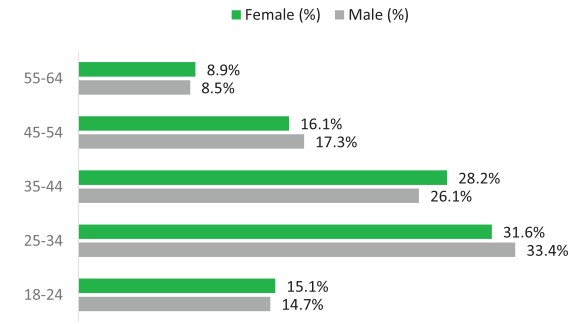
\includegraphics[width=14cm, height=7cm]{umurPC2013} 
	\caption[Komposisi perceived capabilities untuk selang usia yang berbeda]{Komposisi perceived capabilities untuk selang usia yang berbeda} 
	\label{fig:PCUmur} 
\end{figure}

Dapat dilihat pada gambar \ref{fig:PCUmur} bahwa Perceived Capabilities (percaya bahwa mereka memiliki kemampuan dan pengalaman dalam memulai usaha baru) tertinggi terletak pada mereka yang berusia 25 sampai 34 tahun. Perceived Capabilities terendah terletak pada mereka yang berada pada usia 55 sampai 64 tahun.

\begin{figure} [H]
	\centering  
	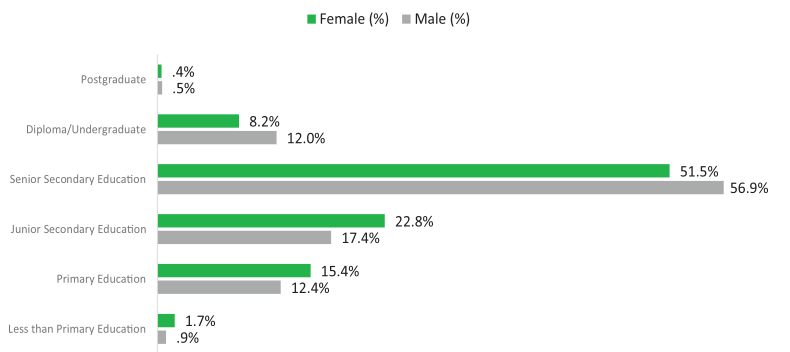
\includegraphics[width=14cm, height=7cm]{pendidikanPC2013} 
	\caption[Komposisi perceived capabilities untuk tingkat pendidikan yang berbeda]{Komposisi perceived capabilities untuk tingkat pendidikan yang berbeda} 
	\label{fig:PCPendidikan} 
\end{figure}

Dapat dilihat pada gambar \ref{fig:PCPendidikan} dijelaskan bahwa individu yang memiliki Perceived Capabilities tertinggi yaitu pada mereka yang telah menyelesaikan Sekolah Menengah Atas. Namun, Perceived Capabilities cenderung rendah bagi mereka yang menyelesaikan pendidikan ditingkat Universitas.

\begin{figure} [H]
	\centering  
	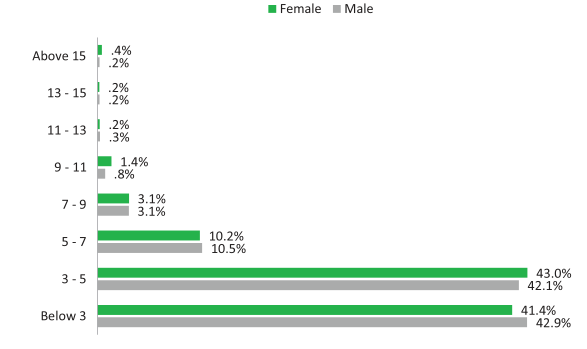
\includegraphics[width=11cm, height=8cm]{pendapatanPC2013} 
	\caption[Komposisi perceived capabilities untuk tingkat pendapatan]{Komposisi perceived capabilities untuk tingkat pendapatan} 
	\label{fig:PCPendapatan} 
\end{figure}


Dapat dilihat pada gambar \ref{fig:PCPendapatan} bahwa Perceived Capabilities tertinggi terletak pada mereka yang memiliki pendapatan di bawah 7 juta. Perceived Capabilities terendah terletak pada mereka yang pendapatannya diatas 11 juta.


\begin{figure} [H]
	\centering  
	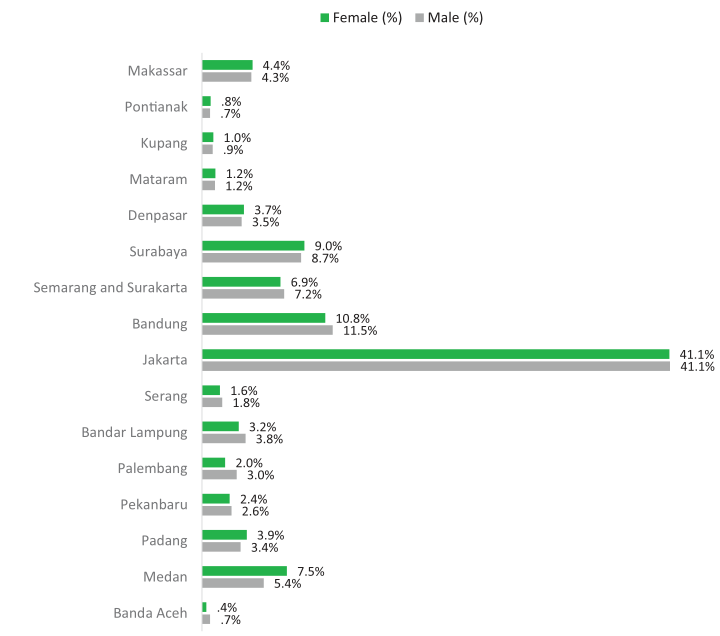
\includegraphics[width=12cm, height=11cm]{lokasiPC2013} 
	\caption[Komposisi perceived capabilities untuk wilayah Indonesia]{Komposisi perceived capabilities untuk wilayah Indonesia} 
	\label{fig:PCRegion} 
\end{figure}


Dapat dilihat pada gambar \ref{fig:PCRegion} dijelaskan bahwa Jakarta memperoleh Perceived Capabilities tertinggi yang artinya banyak orang di Jakarta yang percaya memiliki kemampuan, pengetahuan dan pengalaman untuk memulai usaha baru. Sedangkan Banda Aceh memperoleh Perceived Capabilities terendah untuk wanita sebesar 0.4\% dan untuk pria memiliki dua wilayah yang Perceived Capabilitiesnya rendah yaitu Pontianak dan Banda Aceh masing-masing sebesar 0.7\%.
	\item Data Role Model
\begin{figure} [H]
	\centering  
	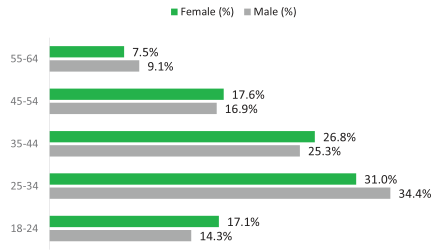
\includegraphics[width=12cm, height=7cm]{umurRM2013} 
	\caption[Komposisi role model untuk umur]{Komposisi role model untuk umur} 
	\label{fig:RMUmur} 
\end{figure}


Pada gambar \ref{fig:RMUmur} dijelaskan individu yang memahami Role Model tertinggi yaitu oleh pria pada selang umur 25 sampai 34 tahun sebesar 34.4\% sedangkan untuk wanita sebesar 31.0\%. Pemahaman Role Model terendahnya yaitu pada selang waktu 55 sampai 64 tahun yang masing-masing nilainya yaitu pria 9.1\% dan wanita 7.5\%.


\begin{figure} [H]
	\centering  
	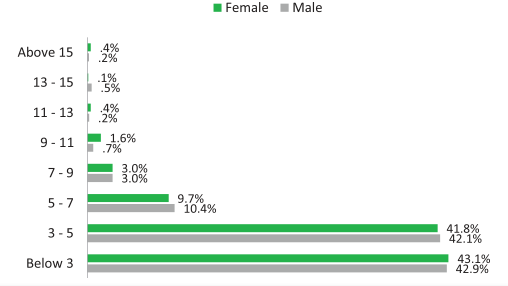
\includegraphics[width=13cm, height=7cm]{pendapatanRM2013} 
	\caption[Komposisi role model untuk tingkat pendapatan yang berbeda]{Komposisi role model untuk tingkat pendapatan yang berbeda} 
	\label{fig:RMpendapatan} 
\end{figure}  


Pada gambar \ref{fig:RMpendapatan} dijelaskan Role Model memiliki peran penting terhadap tingkat pendapatan dibawah 7 juta rupiah. Pada tingkat pendapatan di atas 15 juta rupiah, wanita lebih mempertimbangkan Role Model dibandingkan pria.
	\item Data Perceived Opportunities
\begin{figure} [H]
	\centering  
	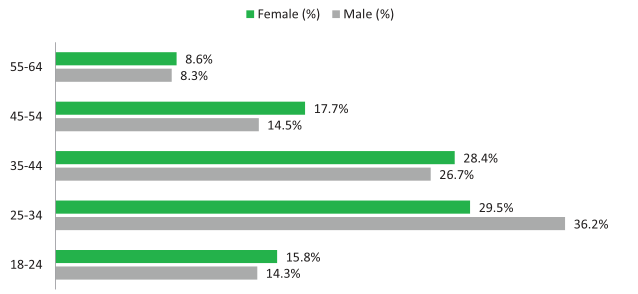
\includegraphics[width=12cm, height=6cm]{umurPO2013} 
	\caption[Komposisi Perceived Opportunities usia wanita dan pria]{Komposisi Perceived Opportunities usia wanita dan pria} 
	\label{fig:POUmur} 
\end{figure} 

Seperti dapat dilihat pada gambar \ref{fig:POUmur}, diantara semuanya yang melihat adanya peluang baik untuk memulai usaha baru yaitu pria berusia antara 25 sampai 34 tahun sebesar 36.2\%, nilai untuk pria memiliki nilai lebih tinggi dibandingkan wanita. Sedangkan pada umur di atas 34 tahun, wanita memiliki nilai yang lebih tinggi dibandingkan pria.

\begin{figure} [H]
	\centering  
	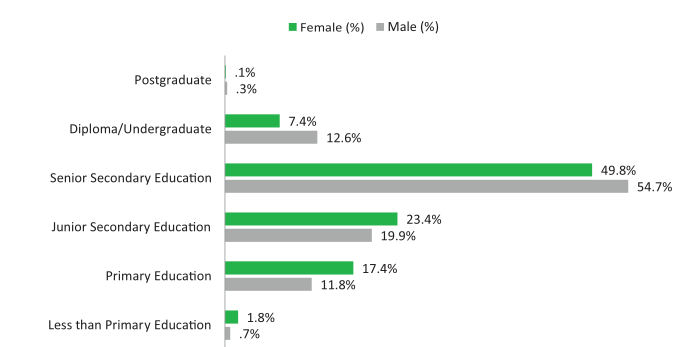
\includegraphics[width=14cm, height=7cm]{pendidikanPO2013} 
	\caption[Komposisi perceived opportunities untuk tingkat pendidikan yang berbeda]{Komposisi perceived opportunities untuk tingkat pendidikan yang berbeda} 
	\label{fig:POpendidikan} 
\end{figure}  

Gambar \ref{fig:POpendidikan} menjelaskan yang memiliki Perceived Opportunities tertinggi yaitu mereka yang menyelesaikan pendidikannya di sekolah menengah atas, komposisi nilai untuk pria lebih tinggi dibandingkan wanita. Perceived Opportunities akan semakin menurun jika tingkat pendidikannya semakin tinggi.

\begin{figure} [H]
	\centering  
	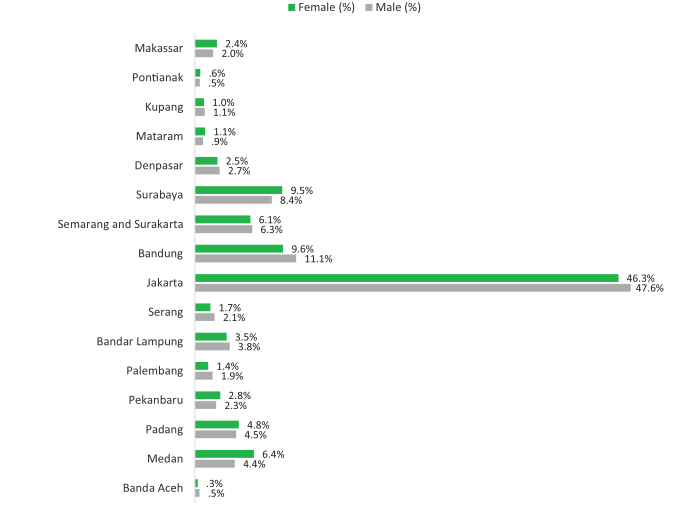
\includegraphics[width=15cm, height=11cm]{lokasiPO2013} 
	\caption[Komposisi Perceived Opportunities untuk wilayah Indonesia]{Komposisi Perceived Opportunities untuk wilayah Indonesia} 
	\label{fig:lokasiPO} 
\end{figure}  

Gambar \ref{fig:lokasiPO} menjelaskan bahwa orang-orang yang tinggal di wilayah Jakarta memiliki Perceived Opportunities tertinggi dibandingkan kota-kota yang lain. Perceived Opportunities cenderung rendah pada wilayah-wilayah di luar pulau Jawa seperti pada wilayah Banda Aceh dan Pontianak.

\begin{figure} [H]
	\centering  
	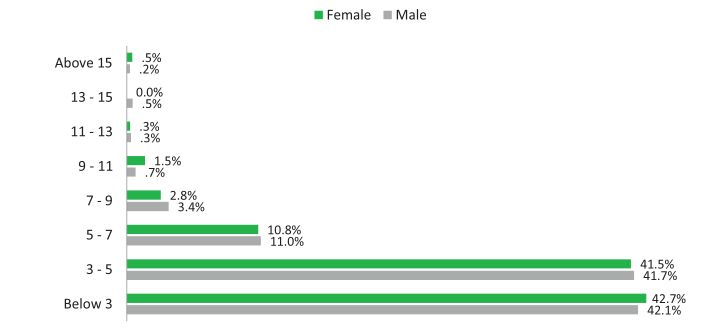
\includegraphics[width=14cm, height=7cm]{pendapatanPO2013} 
	\caption[Komposisi Perceived Opportunities untuk tingkat pendapatan]{Komposisi Perceived Opportunities untuk tingkat pendapatan} 
	\label{fig:pendapatanPO} 
\end{figure} 

Gambar \ref{fig:pendapatanPO} memperlihatkan bahwa mereka yang pendapatannya di bawah 7 juta rupiah memiliki Perceived Opportunities lebih tinggi dibandingkan pendapatan di atas 7 juta rupiah. Rata-rata, wanita dengan pendapatan lebih dari 15 juta rupiah lebih bisa melihat adanya kesempatan memulai usaha baru dibandingkan pria.
	\item Data Fear of Failure
\begin{figure} [H]
	\centering  
	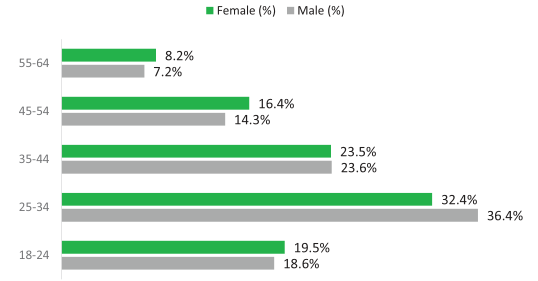
\includegraphics[width=13cm, height=6cm]{usiaFF2013} 
	\caption[Komposisi Fear of Failure untuk usia wanita dan pria]{Komposisi Fear of Failure untuk usia wanita dan pria} 
	\label{fig:umurFF} 
\end{figure} 

Dapat dilihat pada gambar \ref{fig:umurFF}, Fear of Failure tertinggi dimiliki oleh pria berumur antara 25 sampai 34 tahun. Wanita pada usia di atas 44 tahun memiliki Fear of Failure lebih tinggi dibandingkan pria.

\begin{figure} [H]
	\centering  
	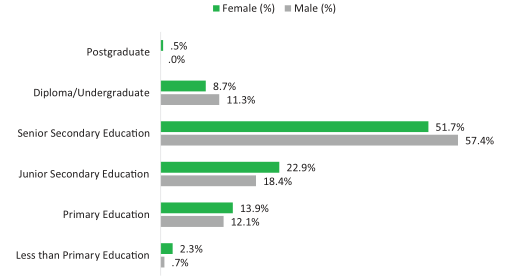
\includegraphics[width=13cm, height=7cm]{pendidikanFF2013} 
	\caption[Komposisi Fear of Failure untuk tingkat pendidikan]{Komposisi Fear of Failure untuk tingkat pendidikan} 
	\label{fig:pendidikanFF} 
\end{figure} 

Pada gambar \ref{fig:pendidikanFF}, Fear of Failure tertinggi dimiliki oleh mereka yang menyelesaikan pendidikannya pada sekolah menengah atas. Semakin tinggi tingkat pendidikan, Fear of Failure menjadi menurun.

\begin{figure} [H]
	\centering  
	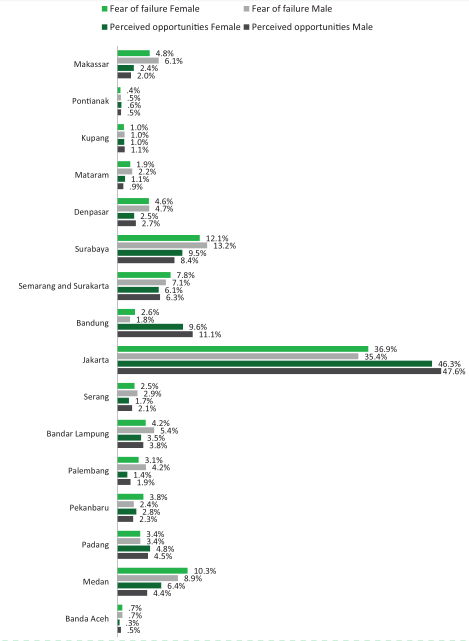
\includegraphics[width=14cm, height=17cm]{lokasiFF2013} 
	\caption[Komposisi Fear of Failure untuk wilayah Indonesia]{Komposisi Fear of Failure untuk wilayah Indonesia} 
	\label{fig:lokasiFF} 
\end{figure} 

Pada gambar \ref{fig:lokasiFF}, sama seperti faktor psikologis lainnya ibukota Indonesia yaitu Jakarta menjadi nilai tertinggi untuk Fear of Failure daripada kota-kota lainnya.
	\item Data High Status of Successful

\begin{figure} [H]
	\centering  
	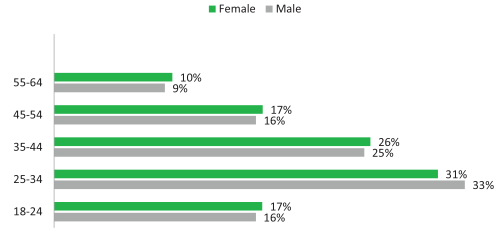
\includegraphics[width=14cm, height=6cm]{umurHS2013} 
	\caption[Komposisi High Status of Successful untuk kategori usia]{Komposisi High Status of Successful untuk kategori usia} 
	\label{fig:umurHS} 
\end{figure} 

Dilihat pada gambar \ref{fig:umurHS}, individu pada usia 25 sampai 34 tahun memiliki persepsi positif bahwa pengusaha yang sukses dihormati dan bercitra tinggi.

\begin{table} [H]
\centering
\caption{Komposisi High Status of Successful untuk tingkat pendidikan}
\begin{tabular}{|c|c|c|}
\hline
Tingkat Pendidikan & Pria & Wanita\\
\hline
Tidak Tamat Pendidikan Dasar & 1\% & 2\%\\
\hline
Pendidikan Dasar & 12\% & 15\%\\
\hline
Pendidikan Menengah Awal & 19\% & 23\%\\
\hline
Pendidikan Menengah Lanjutan & 56\% & 52\%\\
\hline
Diploma & 11\% & 8\%\\
\hline
Pascasarjana & 0\% & 0\%\\
\hline
\end{tabular}
\label{pendidikanHS}
\end{table}

Pada tabel \ref{pendidikanHS}, dapat dievaluasi bahwa wanita dengan tingkat pendidikan rendah memiliki persepsi lebih tinggi bahwa pengusaha yang sukses akan dihormati. Untuk mereka yang berada pada tingkat pendidikan menengah lanjutan, pria memiliki persepsi lebih tinggi mengenai hal tersebut daripada wanita.

\begin{figure} [H]
	\centering  
	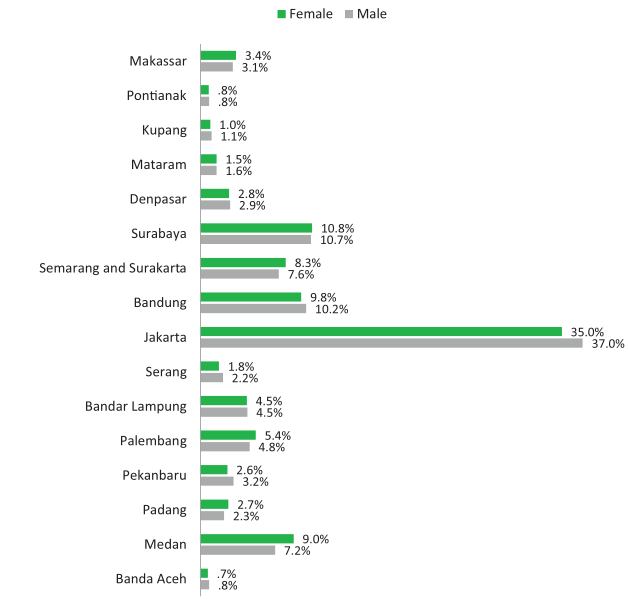
\includegraphics[width=11cm, height=13cm]{lokasiHS2013} 
	\caption[Komposisi High Status of Successful berdasarkan kota tinggal]{Komposisi High Status of Successful berdasarkan kota tinggal} 
	\label{fig:lokasiHS} 
\end{figure} 

Pada gambar \ref{fig:lokasiHS}, orang-orang yang tinggal di kota Jakarta memiliki persepsi lebih tinggi mengenai pengusaha sukses memiliki status tinggi. Selanjutnya akan diteruskan oleh kota Bandung, Surabaya, dsb. Kota yang berada diluar pulau Jawa memiliki persepsi rendah dibandingkan kota-kota yang ada di pulau Jawa.

\begin{figure} [H]
	\centering  
	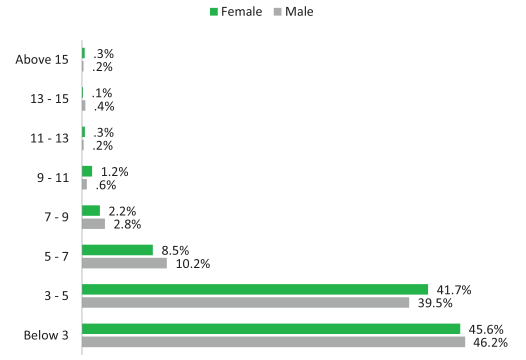
\includegraphics[width=11cm, height=8cm]{pendapatanHS2013} 
	\caption[Komposisi High Status of Successful berdasarkan tingkat pendapatan]{Komposisi High Status of Successful berdasarkan tingkat pendapatan} 
	\label{fig:pendapatanHS} 
\end{figure} 

Dapat dilihat pada gambar \ref{fig:pendapatanHS}, orang-orang dengan pendapatan di bawah 7 juta rupiah memiliki persepsi lebih tinggi mengenai High Status of Successful dibandingkan mereka yang memiliki pendapatan lebih dari 7 juta rupiah. Data selanjutnya yaitu dari Media Attention.
	
	\item Data Media Attention
\begin{figure} [H]
	\centering  
	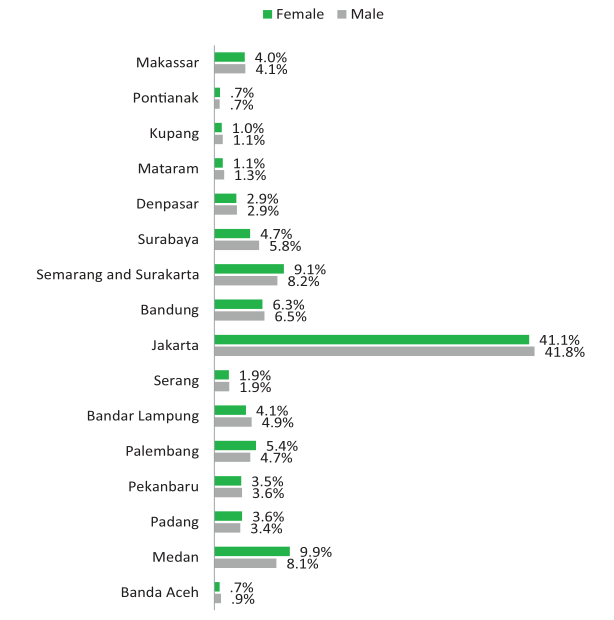
\includegraphics[width=12cm, height=11cm]{lokasiPMA2013} 
	\caption[Komposisi Media Attention berdasarkan kota tinggal]{Komposisi Media Attention berdasarkan kota tinggal} 
	\label{fig:lokasiPMA} 
\end{figure} 

Dilihat pada gambar \ref{fig:lokasiPMA}, dapat disimpulkan walaupun orang-orang yang berada di Jakarta memiliki persepsi lebih tinggi pada niat media untuk melaporkan cerita usaha yang sukses, persepsi tertinggi kedua justru terletak pada daerah di luar pulau jawa yaitu kota Medan.

\begin{figure} [H]
	\centering  
	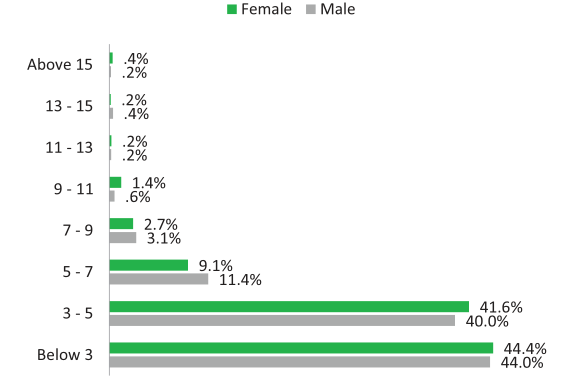
\includegraphics[width=12cm, height=7cm]{pendapatanPMA2013} 
	\caption[Komposisi Media Attention berdasarkan tingkat pendapatan]{Komposisi Media Attention berdasarkan tingkat pendapatan} 
	\label{fig:pendapatanPMA} 
\end{figure} 

Pada gambar \ref{fig:pendapatanPMA}, dapat disimpulkan bahwa mereka yang memiliki pendapatan di bawah 7 juta rupiah memiliki persepsi lebih tinggi pada niat media untuk melaporkan cerita usaha yang sukses dibandingkan dengan mereka yang memiliki pendapatan di atas 7 juta rupiah.
\end{enumerate}
\section{Cellular Automata}
\label{sec:cellularautomata}

Cellular Automata (CA) diperkenalkan pertama kali oleh Ulam dan von Neumann pada tahun 1940. Cellular Automata sendiri merupakan model matematis untuk sistem yang terdapat banyak komponen sederhana bertindak bersama untuk menghasilkan pola perilaku yang rumit \cite{referensiCA2}. Sebuah CA terdiri atas sekumpulan sel, tersusun dalam larik-larik (\textit{grid}). Setiap sel mempunyai satu dari sejumlah \textit{state} (kondisi) yang mungkin. \textit{State} dapat berubah sesuai dengan aturan tertentu. Perubahan \textit{state} dari sebuah sel dipengaruhi oleh \textit{state} dari sel-sel di sekitarnya atau disebut dengan sel tetangga.

\subsection{Dimensi CA}
		\begin{enumerate}
			\item CA Satu Dimensi
			
				\begin{figure} [H]
					\centering  
					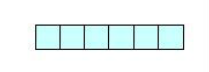
\includegraphics[width=4cm, height=2cm]{CA1D} 
					\caption[CA 1 Dimensi]{CA 1 Dimensi} 
					\label{fig:CA1D} 
				\end{figure}
			
			Cellular Automata satu dimensi adalah cellular automata yang ruang selnya berupa array satu dimensi, sehingga masing-masing sel hanya memiliki dua tetangga yang tepat bersebelahan, kecuali sel paling pinggir yang hanya mempunyai satu tetangga. CA satu dimensi biasanya memakai aturan yang diusulkan oleh Wolfram. Sebagai contoh berikut aturan no. 30 diberikan pada gambar \ref{fig:wolfram}
			
			
			\begin{figure} [H]
					\centering  
					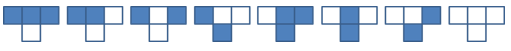
\includegraphics[width=10cm, height=2cm]{wolfram} 
					\caption[Aturan 30 dari Wolfram]{Aturan 30 dari Wolfram} 
					\label{fig:wolfram} 
				\end{figure}
				
				Cara membaca aturan tersebut adalah pada baris pertama terdapat 3 sel pada suatu saat (iterasi) tertentu, sel yang ditinjau adalah sel yang berada di tengah. Tetangga dari sel tersebut yaitu tetangga kiri dan kanan. Baris kedua menunjukkan keadaan sel pada \textit{state} berikutnya. Sebagai contoh pada gambar paling kiri, sel pada bagian tengah (gelap) mempunyai tetangga kiri gelap dan tetangga kanan gelap maka iterasi berikutnya \textit{state} sel tersebut berubah menjadi putih.
				
				Sebagai ilustrasi, pada gambar \ref{fig:penerapanwolfram} diberikan contoh penerapan aturan 30 dari Wolfram yang dimulai dari kondisi awal (t=0) dengan sel gelap yang berada di tengah hingga t=9. \cite{ECA}
				
				\begin{figure} [H]
					\centering  
					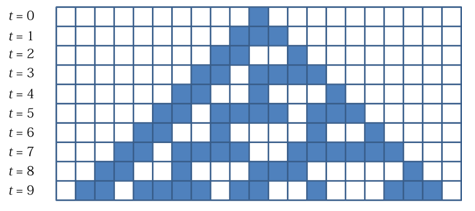
\includegraphics[width=10cm, height=6cm]{penerapanwolfram} 
					\caption[Ilustrasi penerapan aturan 30 dari Wolfram]{Ilustrasi penerapan aturan 30 dari Wolfram} 
					\label{fig:penerapanwolfram} 
				\end{figure}
				
			\item CA Dua Dimensi
			
			\begin{figure} [H]
					\centering  
					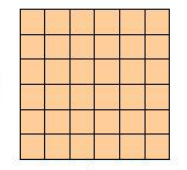
\includegraphics[width=4cm, height=2cm]{CA2D} 
					\caption[CA 2 Dimensi]{CA 2 Dimensi} 
					\label{fig:CA2D} 
				\end{figure}
			
			Cellular Automata dua dimensi adalah cellular automata yang ruang selnya biasanya berupa matriks, sehingga masing-masing sel memiliki lebih dari dua tetangga. CA dua dimensi yang sangat terkenal adalah Conway's \textit{Game of Life}. Setiap sel pada CA menggambarkan suatu individu yang dapat berada pada \textit{state} hidup atau mati. Sel hidup dapat berubah menjadi mati dan sel mati dapat berubah menjadi sel hidup. Aturan dasar Conway's diberikan pada gambar \ref{fig:conway}
			
			
			\begin{figure} [H]
					\centering  
					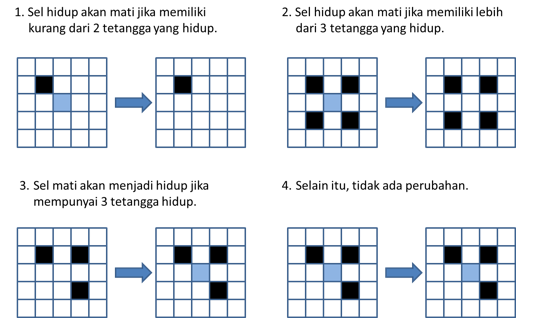
\includegraphics[width=12cm, height=8cm]{conway} 
					\caption[Aturan Dasar Conway's Game of Life]{Aturan Dasar Conway's Game of Life} 
					\label{fig:conway} 
				\end{figure}
			
			Berikut ilustrasi Conway yang menggambarkan perubahan yang terjadi pada sekumpulan sel mulai dari kondisi awal (t=0) sampai dengan kondisi akhir (t=3) yang dilakukan secara iteratif. Banyaknya sel hidup pada kondisi awal berkurang sedikit demi sedikit sampai pada kondisi akhir tidak ada lagi sel hidup. \cite{ECA}
			
			
			\begin{figure} [H]
					\centering  
					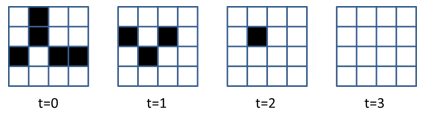
\includegraphics[width=10cm, height=3cm]{contohconway} 
					\caption[Ilustrasi Conway's Game of Life]{Ilustrasi Conway's Game of Life} 
					\label{fig:contohconway} 
				\end{figure}
			
\end{enumerate}		
\subsection{Aplikasi CA} 
		
		\begin{enumerate}
			\item Bidang Transportasi
			
			CA banyak digunakan untuk memodelkan lalu lintas, dengan tujuan utama biasanya adalah untuk mempelajari beban dari jalan-jalan di area tertentu. Contoh aplikasi CA dibidang transportasi ini adalah simulasi pengaturan lampu lalu lintas. Model dalam penelitian ini menggunakan CA 1 dimensi.
			
			\item Bidang Kesehatan
			
			Pada bidang kesehatan, CA juga sering digunakan untuk pemodelan penyebaran penyakit. Biasanya masalah penyebaran penyakit dimodelkan dengan CA dua dimensi dan menggunakan aturan Game of Life dari Conway. Contoh aplikasi yang diterapkan di dunia nyata yaitu simulasi infeksi virus influenza A menggunakan cellular automaton. Pada penelitian ini cellular automata yang digunakan adalah CA dua dimensi. CA yang dibangun akan memodelkan CA yang memiliki \textit{lattice} berbentuk segienam sebagai penyederhanaan dari bentuk bola ke dalam dua dimensi, hal ini dikarenakan sel tubuh manusia berbentuk seperti bola. Pada penelitian ini digunakan batasan secara \textit{periodic}, dengan asumsi sel yang berseberangan sebenarnya bersebelahan pada kondisi aslinya karena masing-masing virus hanya dapat menginfeksi jaringan tubuh tertentu saja. \cite{referensiCA1}
			
			\item Bidang Lingkungan / Ekologi
			
			CA juga dapat digunakan untuk pemodelan pada bidang lingkungan. Contoh penerapan cellular automata pada bidang lingkungan adalah simulasi dan pemodelan perubahan penggunaan lahan. Penelitian ini menggunakan algoritma DINAMICA, algoritma ini merupakan algoritma cellular automata hibrida yang mendukung pemodelan statistik untuk menemukan area yang berpotensi mengalami perubahan berdasarkan faktor pemicu yang telah ditentukan.
			
			\item Bidang Sains
			
			Pada bidang sains, khususnya fisika CA dapat digunakan untuk memodelkan pergerakan partikel dan juga permasalahan lainnya terkait dengan fisika kuantum. Pada bidang biologi, CA digunakan untuk memodelkan sel biologis.
		\end{enumerate}
		


\section{Entrepreneurial Cellular Automata}
\label{sec:ECA}
\textit{Entrepreneurial Cellular Automata} merupakan pengembangan model dari \textit{Cellular Automata} yang digunakan untuk mensimulasikan pertumbuhan kewirausahaan di Indonesia. Dalam kasus \textit{Entrepreneurial Cellular Automata} (ECA), sel akan merepresentasikan wirausahawan dan ketetanggaannya akan merepresentasikan hubungan antar wirausahawan. Setiap wirausahawan mempunyai dua sifat atribut yaitu statis (nilainya tidak berubah) dan dinamis (nilainya dapat berubah). Contoh atribut statis adalah bidang usaha, kategori usaha, lokasi geografis dan jenis kelamin. Contoh atribut dinamis adalah usia, level wirausaha dan usia usaha.  

Perubahan atribut dinamis dari waktu ke waktu didefinisikan dengan fungsi transisi. Fungsi transisi terdiri dari beberapa aturan. Atribut penting dalam kewirausahaan yaitu level wirausaha karena atribut ini digunakan untuk menentukan perkembangan dari kewirausahaan. Cara menentukan seorang wirausaha akan meneruskan usahanya diketahui dari sebuah angka yang disebut \textit{Continuity Index} (CIdx). CIdx dari seorang wirausaha tidak hanya dipengaruhi oleh faktor dari dalam tetapi juga dipengaruhi oleh faktor dari luar. Faktor luar dipengaruhi oleh tetangganya dan faktor publik seperti kebijakan pemerintah, kondisi perekonomian dunia, dsb. Seorang wirausahawan akan meneruskan usahanya jika CIdx-nya memenuhi nilai ambang tertentu.

Atribut dari seorang wirausahawan dapat berubah dari waktu ke waktu, hal ini menyebabkan ketetanggaan juga dapat berubah dari waktu ke waktu. Sebagai contoh, diasumsikan terdapat wirausahawan $e1$ dan $e2$ bertetanggaan pada waktu $t$, jika $e1$ berubah keadaannya pada $t+1$ maka $e1$ dan $e2$ tidak lagi bertetanggaan pada saat $t+1$.

Berikut definisi ECA :\\
Diberikan \textit{p} himpunan nilai atribut: $A_{1}, ..., A_{p}$ dan sebuah indikator $Pub$ = ${p_{1}, ..., p_{m}}$, sebuah ECA $M$ adalah sebuah tupel
\begin{displaymath}
	M = (E, \alpha, N, \omega, \rho, \delta, \sigma)
\end{displaymath}
dimana :
\begin{itemize}
	\item $E = {e_{1}, ..., e_{n}}$ adalah himpunan berhingga wirausahaan,
	\item $\alpha = {\alpha_{1}, ..., \alpha_{p}}$ adalah himpunan berhingga atribut dimana setiap $\alpha_{i}$ didefinisikan sebagai $\alpha_{i} : E \rightarrow A_{i}$,
	\item $N = {N_{1}, ..., N_{k}}$ adalah himpunan berhingga ketetanggaan dimana setiap $N_{i}$ didefinisikan sebagai $N_{i}:E \times E \rightarrow \Re$,
	\item $\omega = {\omega_{1}, ..., \omega_{k}}$ adalah himpunan fungsi bobot atau nilai ketetanggaan dimana $\omega_{i} : N_{i} \rightarrow \Re$ memetakan setiap fungsi ketetanggaan ke sebuah bilangan riil,
	\item $\rho = {\rho_{1}, ..., \rho_{p}}$ adalah himpunan indikator publik dimana setiap $\rho_{i}$ didefinisikan sebagai $\rho_{i} : p_{i} \rightarrow \Re$,
	\item $\delta : \beta \rightarrow \beta$ adalah fungsi transisi state, dan
	\item $\sigma : N \rightarrow N$ adalah sebuah fungsi transformasi ketetanggaan.
\end{itemize}


Berdasarkan model kewirausahaan terdapat empat tingkatan wirausaha yaitu \textit{potential}, \textit{nascent}, \textit{new business manager} dan \textit{manager of established business}. Akan ditambahkan pula tingkatan wirausaha yang menyatakan wirausahawan di atas umur 64 tahun yaitu \textit{retired}. Pada gambar \ref{fig:tingkatwirausaha} akan ditunjukkan secara lebih lanjut, \textit{new\_bm} dan \textit{est\_bm} dinyatakan sebagai \textit{new business manager} dan \textit{manager of established business}.


	\begin{figure} [H]
		\centering  
		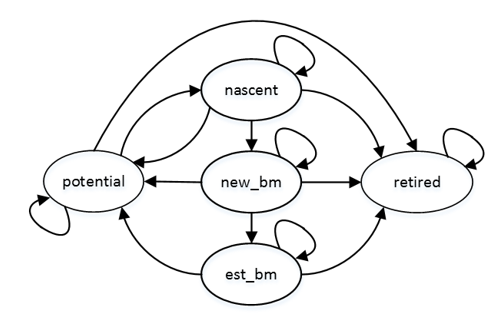
\includegraphics[width=9cm, height=5cm]{tingkatwirausaha} 
		\caption[Diagram Transisi Level Wirausaha]{Diagram Transisi Level Wirausaha} 
		\label{fig:tingkatwirausaha} 
	\end{figure}


\section{Graf}
\label{sec:graf}
Graf dalam matematika dan ilmu komputer adalah himpunan benda-benda yang disebut simpul (\textit{vertex} atau \textit{node}) yang terhubung oleh sisi (\textit{edge}). Sebuah graf biasanya digambarkan dengan sekumpulan titik-titik yang dihubungkan oleh garis-garis. Suatu sisi dapat menghubungkan suatu simpul dengan simpul yang sama, sisi ini disebut dengan \textit{loop}.

Graf biasanya dinyatakan sebagai $G = <V,E>$, dimana V adalah simpul pada graf sedangkan E adalah sisi pada graf. Sebagai contoh definisi dari graf terdapat $V = {A,B,C,D,E,F,G,H,I}$ dan $E = {{A,B},{A,C},{B,D},{C,D},{C,E},{E,F},{E,G},{H,I}}$ berikut gambar graf sesuai dengan pernyataan V dan E di atas :

	\begin{figure} [H]
		\centering  
		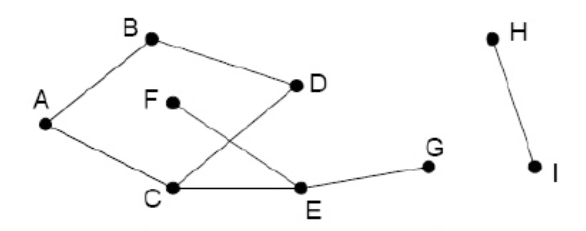
\includegraphics[width=8cm, height=4cm]{graf5} 
		\label{fig:graf5} 
	\end{figure}
	
Graf memiliki banyak jenis, jenis-jenis graf ini didasarkan pada ada tidaknya \textit{loop} pada suatu graf dan sisi pada graf yang mempunyai orientasi arah. Berdasarkan ada tidaknya \textit{loop} pada suatu graf digolongkan menjadi dua jenis :
\begin{enumerate}
	\item Graf Sederhana
	
	Graf ini tidak mempunyai sisi ganda.
	\item Graf tak-sederhana
	
	Graf ini mempunyai sisi ganda.
\end{enumerate}

Berdasarkan orientasi arah pada sisi, secara umum graf dibedakan menjadi 2 jenis :
\begin{enumerate}
	\item Graf tak-berarah
	
	Graf yang sisinya tidak mempunyai arah. Pada graf ini urutan sisi tidak diperhatikan.
	\item Graf berarah
	
	Graf yang sisinya mempunyai arah. Pada graf ini urutan sisi diperhatikan. \cite{referensiCA5}
\end{enumerate}

Sebuah graf dinyatakan sebagai struktur data yang terdiri dari simpul dan sisi yang membangun hubungan antar simpul. Terdapat dua macam representasi graf yaitu \textit{adjacency list} dan \textit{adjacency matrix}. \cite{referensiGraph1}
\subsection{Adjacency List}
Adjacency list merupakan bentuk representasi dari seluruh sisi dalam sebuah graf sebagai suatu senarai (\textit{linked list}). Simpul-simpul yang dihubungkan merupakan simpul-simpul yang saling terkait. Dalam implementasinya, adjacency list menggunakan \textit{hash table} untuk menghubungkan satu simpul dengan simpul lain yang saling terkait. Contoh implementasi adjacency list yaitu sebagai berikut :

 	\begin{figure} [H]
		\centering  
		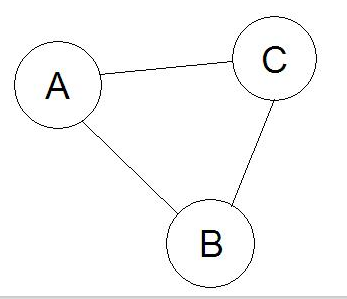
\includegraphics[width=4cm, height=4cm]{adjacencylist} 
		\caption[\textit{Undirected Cyclic Graph}]{\textit{Undirected Cyclic Graph}}
		\label{fig:GambarAL} 
	\end{figure}
	
	Graf pada gambar \ref{fig:GambarAL} dapat direpresentasikan melalui tabel \ref{tabelAL} :
	
	
	\begin{table}[H]
\centering
\caption{Tabel Representasi Adjacency List}
\begin{tabular}{|c|p{2cm}|c|}
\hline
Vertex & Adjacency & Array of Adjacent\\
\hline
a & adjacent to & b,c \\
\hline
b & adjacent to & a,c \\
\hline
c & adjacent to & a,b\\
\hline
\end{tabular}
\label{tabelAL}
\end{table}

\subsection{Adjacency Matrix}
Adjacency Matrix merupakan representasi matrix $N \times N$ yang menyatakan hubungan antar simpul dalam suatu graf. Kolom dan baris menyatakan simpul-simpul, sedangkan nilai entri dari matrix menyatakan hubungan antar simpul. Contoh implementasi adjacency matrix pada graf tidak berarah yaitu sebagai berikut :

\begin{figure} [H]
		\centering  
		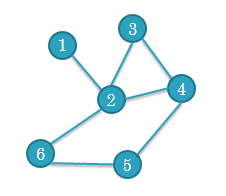
\includegraphics[width=5cm, height=4cm]{adjacencymatrix} 
		\caption[\textit{Undirected Cyclic Graph}]{\textit{Undirected Cyclic Graph}}
		\label{fig:GambarAM} 
	\end{figure}


Graf pada gambar \ref{fig:GambarAM} dapat direpresentasikan melalui tabel \ref{tabelAM} :


\begin{table}[H]
\centering
\caption{Tabel Representasi Adjacency Matrix}
\begin{tabular}{|c|c|c|c|c|c|c|}
\hline
v & 1 & 2 & 3 & 4 & 5 & 6 \\
\hline
1 & 0 & 1 & 0 & 0 & 0 & 0 \\
\hline
2 & 1 & 0 & 1 & 1 & 0 & 1 \\
\hline
3 & 0 & 1 & 0 & 1 & 0 & 0 \\
\hline
4 & 0 & 1 & 1 & 0 & 1 & 0 \\
\hline
5 & 0 & 0 & 0 & 1 & 0 & 1 \\
\hline
6 & 0 & 1 & 0 & 0 & 1 & 0 \\
\hline
\end{tabular}
\label{tabelAM}
\end{table}

Contoh adjacency matrix pada graf berarah yaitu sebagai berikut :

\begin{figure} [H]
		\centering  
		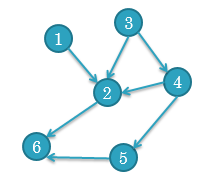
\includegraphics[width=5cm, height=4cm]{graf3} 
		\caption[\textit{Directed Cyclic Graph}]{\textit{Directed Cyclic Graph}}
		\label{fig:GambarDCG} 
	\end{figure}
	
Graf pada gambar \ref{fig:GambarDCG} dapat direpresentasikan melalui tabel \ref{tabelDCG} :

\begin{table}[H]
\centering
\caption{Tabel Representasi Adjacency Matrix}
\begin{tabular}{|c|c|c|c|c|c|c|}
\hline
v & 1 & 2 & 3 & 4 & 5 & 6 \\
\hline
1 & 0 & 1 & 0 & 0 & 0 & 0 \\
\hline
2 & 0 & 0 & 0 & 0 & 0 & 1 \\
\hline
3 & 0 & 1 & 0 & 1 & 0 & 0 \\
\hline
4 & 0 & 1 & 0 & 0 & 1 & 0 \\
\hline
5 & 0 & 0 & 0 & 0 & 0 & 1 \\
\hline
6 & 0 & 0 & 0 & 0 & 0 & 0 \\
\hline
\end{tabular}
\label{tabelDCG}
\end{table}
